\setlength{\footskip}{8mm}


\chapter{Literature Review} 
\label{ch:literature-review}

\textit{This chapter will compare all relevant and previously published material on drones and particularly on drone control. As mentioned in the previous chapter, the ultimate aim of this study is to help a ground control station (GCS) on the web communicate effectively and securely with a fleet of drones. This system will offer a high-level control system for this fleet. Several offline non-web applications already exist, such as QGroundControl and Mission Planner, both of which are open-source.
}

\section{UAV Swarming}

A UAV swarm refers to a group of drones that communicate with each other in flight and can spontaneously react to the situation. These drones usually collaborate on a single task. There are already several papers that focus on drone swarming technology.
\shortciteA{burdoin1996airborne} is one of the earliest – albeit military – proponents of a unified “formation of drones,” in which drones “will sense relative movement parameters.” This study uses a leader-follower approach in which one drone is assigned leader and other drones get data from it.

The modern implementation of this would be much more complex.
Most existing systems seek to control a fleet with a centralized approach, by sending commands to each UAV from a GCS. According to \citeA{dietrich2016towards}, this is inefficient and a more decentralized approach method is proposed. An extension to the existing MAVLink protocol is proposed, adding more messages and also implementing inter-UAV (intra-fleet) communication. For their study, the MAVLink common message set is not sufficient for swarm control and hence the authors also propose a more suitable message set for swarming.


Their proposal even includes additional MAVLink messages for drone repair and battery recharging through so-called “intelligent charging stations (ICS),” although actual implementation would be far more complex. Further research can be done in the field of ICSs.

\begin{figure}[t]
	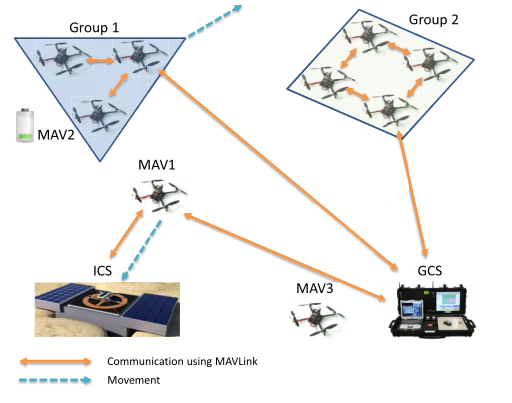
\includegraphics[width=\textwidth]{Ch2/dietrich_mission}
	\caption[An example mission in progress from\protect\shortcite{dietrich2016towards}.]{An example mission in progress from\protect\shortcite{dietrich2016towards}. Reprinted from \protect\shortciteA{dietrich2016towards}.}
	\label{fig:dietrichmission}
\end{figure}
\FloatBarrier

Figure \ref{fig:dietrichmission} shows an example mission consisting of a ground control station, an intelligent charging station, two individual MAVs and two MAV swarms. The system that will be developed in this study is not dissimilar to one depicted above, with the differences being:

\begin{enumerate}
  \item The GCS is moved onto a web interface.
  \item The vehicle in use is a UAV, being larger than a standard MAV.
  \item There will be no support for a swarming feature, although this can be implemented (and might even be desirable for a drone-reliant society) in the future.
\end{enumerate}


\section{MAVLink}\label{sect:mavlink}
MAVLink is a lightweight message protocol for drones that is maintained and updated by the community. It is used in the communication between a GCS and a drone and also between onboard drone components such as cameras, servos, etc. It was first released in 2009 by Lorenz Meier and is now integrated on well-known flight controllers such as Pixhawk, ArduPilot among others. There are two major versions: version 1.0 and 2.0 which is backwards-compatible, with latest being version 2.3. Figure 2.3 shows the structure of a MAVLink packet for version 2.

\begin{figure}[t]
	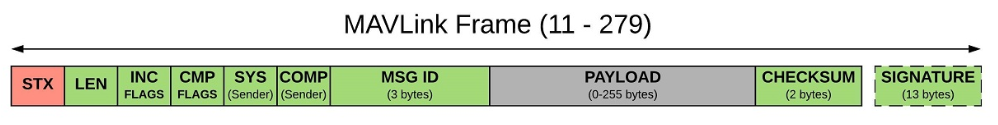
\includegraphics[width=\textwidth]{Ch2/mavlink_v2}
	\caption[MAVLink packet structure.]{MAVLink packet structure. Reprinted from \protect\citeA{meier2013mavlink}.}
	\label{fig:packetstructure}
\end{figure}
\FloatBarrier

% \begin{figure}[h]
% 	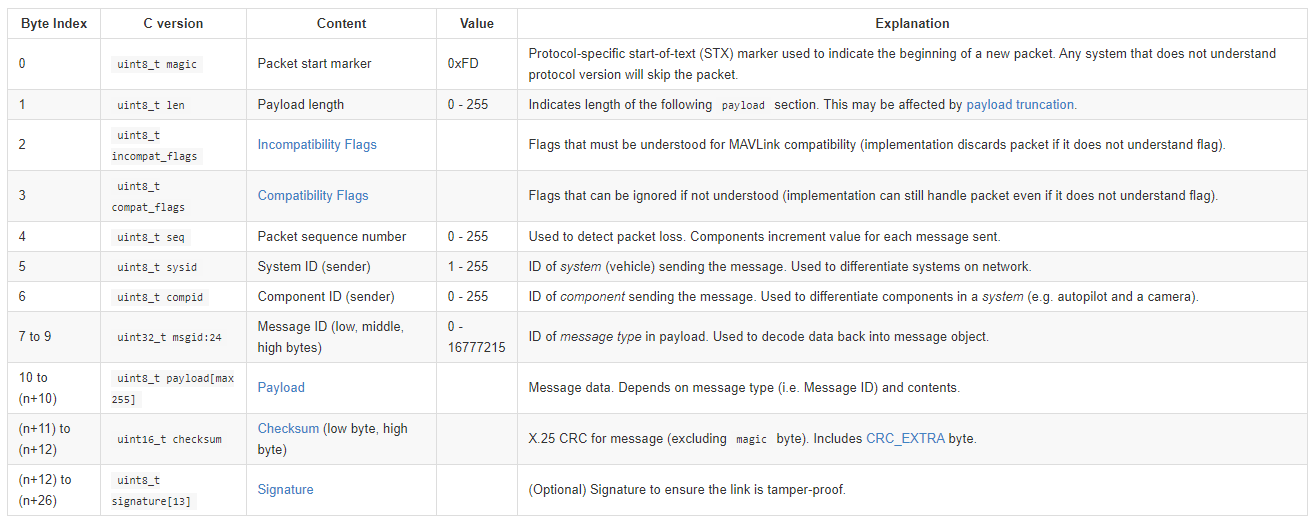
\includegraphics[width=16cm, height=7cm]{Ch2/mavlink_desc}
% 	\caption{MAVLink packet structure. Reprinted from \protect\citeA{meier2013mavlink}.}
% 	\label{fig:packetstructureb}
% \end{figure}
% \FloatBarrier

The MAVLink library provides an extensive collection of messages in the “Common Messages Set”. These provide for a wide range of applications and are sufficient for the purposes of this study. There are over 300 commands and over 300 status messages as well in version 2.3. As explained in the above sections, more messages can be added if this message set is not sufficient enough. 

These messages are defined within XML files and can be accessed on the MAVLink website. Each file's message set are part of a ``dialect'', that is supported by a particular MAVLink system \shortcite{meier2013mavlink}. The most popular reference message set, implemented by the majority of ground control stations and autopilots, is defined in \texttt{common.xml} on the website. Other such ``dialects'' are derived from this definition.

% Messages are defined within XML. Each XML file defines the message set supported by a particular MAVLink system, also referred to as a ``dialect". \shortcite{meier2013mavlink} The reference message set that is implemented by most ground control stations and autopilots is defined in common.xml on the MAVLink website (most dialects build on top of this definition). 

There are two main types of messages - commands and status messages. There is also extensive documentation on the MAVLink type enumerations which are used in the aforementioned commands and status messages. These are all written by \citeA{meier2013mavlink}.


\subsection{Enumerations}\label{sect:enum}

MAVLink enumerations provide enumerated values for certain predefined parameters. These enumerations will be used in the more complex commands and status messages. The example in Figure \ref{fig:enum} below shows the enumerations associated with the type of MAV that will be reported in the HEARTBEAT message (see Figure \ref{fig:heartbeat}).

\begin{figure}[t]
	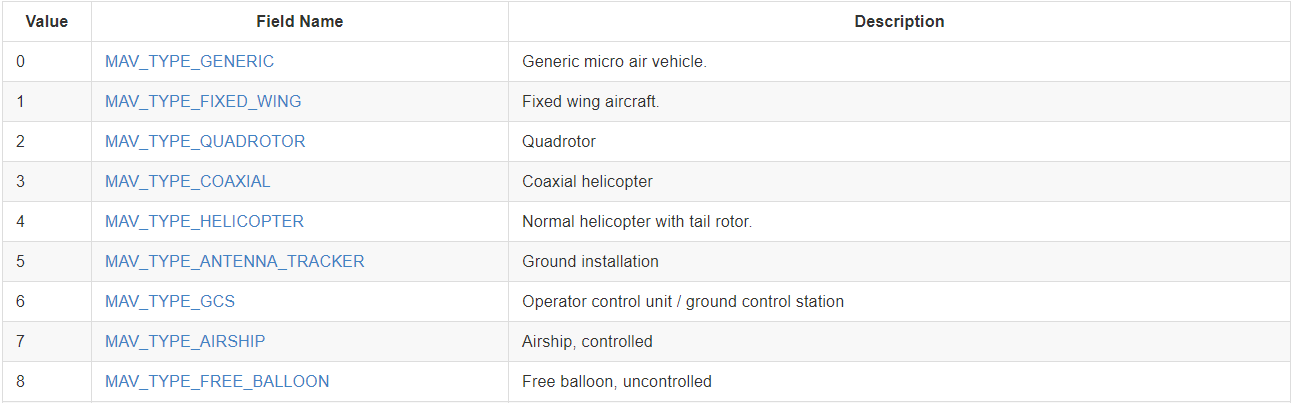
\includegraphics[width=\textwidth]{Ch2/mav_type_enum}
	\caption[MAVLink MAV\_TYPE enumeration.]{MAVLink MAV\_TYPE enumeration. Reprinted from \protect\citeA{meier2013mavlink}.}
	\label{fig:enum}
\end{figure}
\FloatBarrier

\subsection{Commands}\label{subsect:mavlinkcommands}

This section will detail the important MAVLink messages in use in this system. There are three main types of commands - navigation, conditional and do (DO). Out of these, the most important are the navigation commands. DO commands are used to control auxiliary devices, not the drone and conditional commands affect only DO commands.

Navigation commands can be used to control every aspect of the drone’s movements. The most useful of the NAV commands will probably be "MAV\_CMD\_NAV\_WAYPOINT". This simply asks the drone to navigate to the specified location. The location is specified as parameters in the message. This NAV command has seven message parameters and the last three are the target latitude, longitude and altitude that the drone has to follow. Other commands include "MAV\_CMD\_NAV\_TAKEOFF" and "MAV\_CMD\_NAV\_LAND". Figure \ref{fig:waypoint} below shows the MAV\_CMD\_NAV\_WAYPOINT command parameters.

\begin{figure}[t]
	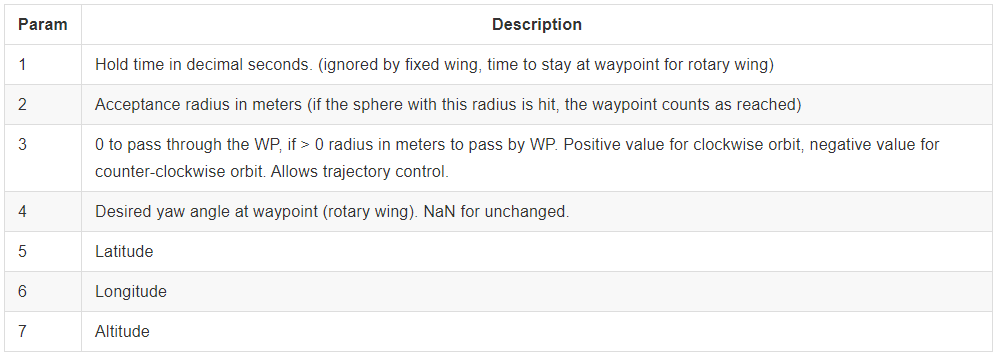
\includegraphics[width=\textwidth]{Ch2/mavlink_nav_waypoint}
	\caption[MAVLink MAV\_CMD\_NAV\_WAYPOINT command.]{MAVLink MAV\_CMD\_NAV\_WAYPOINT command. Reprinted from \protect\citeA{meier2013mavlink}.}
	\label{fig:waypoint}
\end{figure}
\FloatBarrier

\subsection{Messages}

The generic messages set provides a means for the drone to send flight telemetry and status information to the GCS. For example, Figure \ref{fig:heartbeat} below shows the HEARTBEAT message along with accompanying parameters. This implies that the system or component of interest is functioning and responding as intended. The type and autopilot fields (along with the message component id), allow the receiving system to recognize the target system and respond to it appropriately (e.g. by creating the user interface depending on the autopilot). As can be seen, the enumerations in Section \ref{sect:enum} are used.

\begin{figure}[t]
	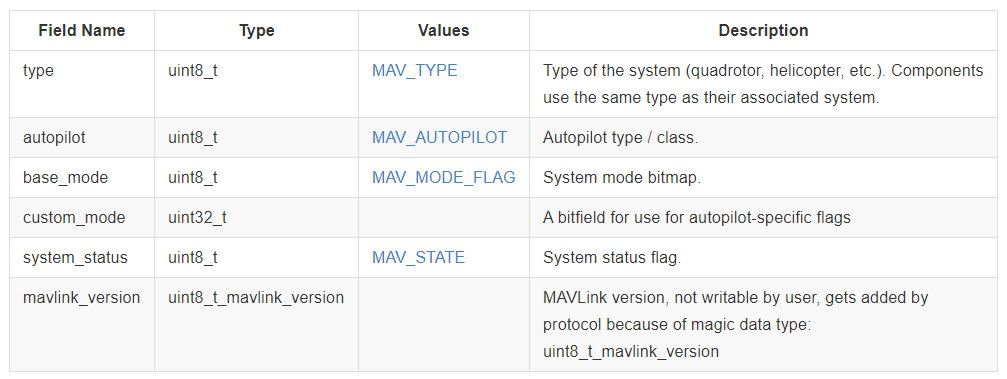
\includegraphics[width=\textwidth]{Ch2/heartbeat_msg}
	\caption[MAVLink HEARTBEAT message.]{MAVLink HEARTBEAT message. Reprinted from \protect\citeA{meier2013mavlink}.}
	\label{fig:heartbeat}
\end{figure}
\FloatBarrier

There are also other messages such as battery information (BATTERY\_STATUS) and flight telemetry information (ATTITUDE, GLOBAL\_POSITION\_INT, etc.)

\subsection{Implementations}
MAVLink is implemented by many autopilot systems (Section  \ref{sect:autopilot}), GCSs (Section  \ref{subsect:gcs}) and even high level APIs \cite{meier2013mavlink}. Most of these are being actively developed. 

\begin{table}[t]
 \caption[MAVlink-supported autopilots and GCSs.]{MAVlink-supported autopilots and GCSs. Data from \protect\citeA{meier2013mavlink}.}
 \begin{center}
     \begin{tabular}{|m{5cm}|m{8cm}|} 
     \hline
     \textbf{Autopilots} & \textbf{Ground Control Stations} \\ [0.5ex] 
     \hline\hline
     PX4 & QGroundControl \\ 
     \hline
     ArduPilot & Mission Planner \\
     \hline
     AutoQuad 6 AutoPilot & MAVProxy\\
     \hline
     iNAV & Side Pilot \\
     \hline
     SmartAP Autopilot & UgCS (Universal Ground Control Station)\\ [1ex] 
     \hline
 \end{tabular}
 \end{center}{}
\end{table}
\FloatBarrier

The standard pre-built MAVLink libraries are sufficient for C/C++ projects, but it is possible to generate MAVLink source files for any other supported language. The supported languages are given below in Figure \ref{fig:lang}:

\begin{figure}[t]
	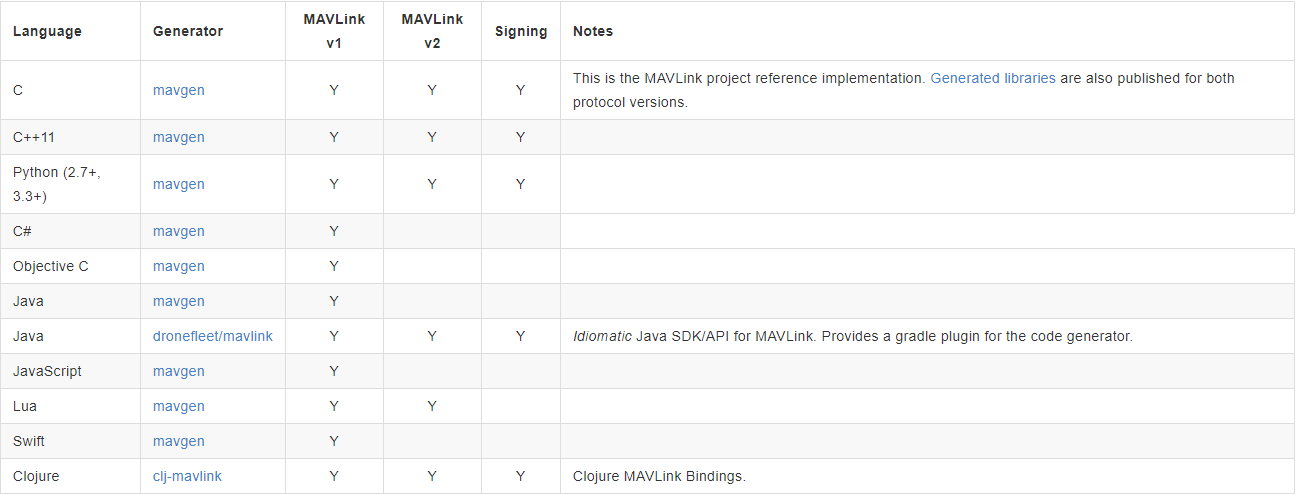
\includegraphics[width=\textwidth]{Ch2/mavlink_lang}
	\caption{MAVLink supported languages. Data from \protect\citeA{meier2013mavlink}.}
	\label{fig:lang}
\end{figure}
\FloatBarrier

There are also several high level developer APIs or wrappers that simplify the process of interacting with MAVLink-enabled components (autopilot, GCSs, etc.). These are available in different languages such as C++ (Dronecode SDK) and Python (Dronekit).

\subsection{MAVLink Security}
Another factor to consider in a UAV communication system is security. \citeA{butcher2013securing} introduced several methods of combating different types of wireless attacks. This brought an effort to encrypt messages in the MAVLink protocol. In this project, SSH will be used to connect to the onboard computer so no encryption is needed on the MAVLink level. The MAVLink messages will be passed directly to the flight controller on the drone.

\section{Management and Control}
\label{management-and-control}

\subsection{Ground Control Stations}
\label{subsect:gcs}
Although UAV technology and usage are on the rise, adequate support software is still rare. This software, along with all supplementary hardware such as telemetry modules, is called a ground control station. According to \citeA{rath2007ground}, a GCS ``includes a management unit, a telemetry module, a user control module, a graphical user interface, and a wireless datalink subsystem.''

However, there have been an increasing number of efforts. For example, a study by \cite{itkin2016development} propose a prototype cloud-based UAV monitoring and management system. Their primary aim is a scalable management system, offering real-time sensor data and collision avoidance for an increasingly drone-reliant world.

\begin{figure}[t]
	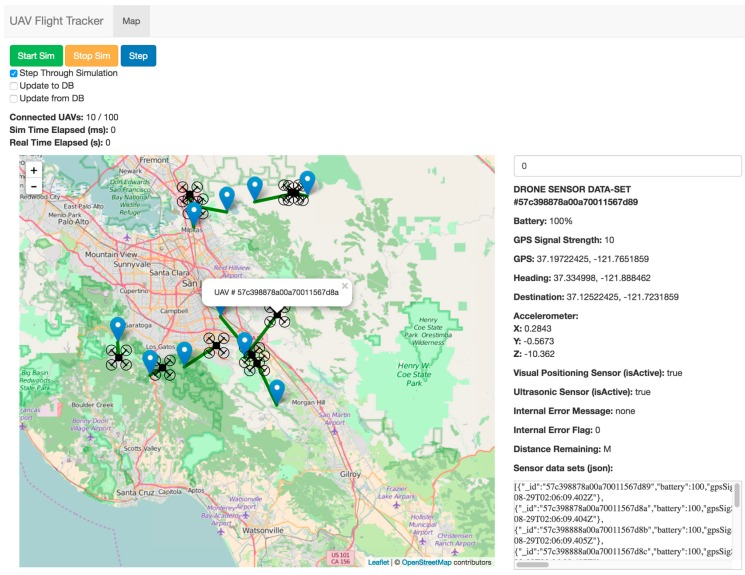
\includegraphics[width=\textwidth]{Ch2/sensors-16-01913-g007}
	\caption[Cloud-based UAV monitoring \protect\cite{itkin2016development}.]{A client interface for cloud-based UAV monitoring. Reprinted from\protect\shortcite{itkin2016development}.}
	\label{fig:clouduav}
\end{figure}
\FloatBarrier

Their system utilizes a server-client topology, in which flight data is stored in a database and accessed in a REST-like architecture. This system is not dissimilar to the ultimate goal of this study but make no mention of the communication itself. Their results focus was on web and server performance.

Yet another study by \citeA{perez2013ground} proposes a ground control station for a multi-UAV surveillance system. It ``allows the operator to dynamically allocate different tasks to the UAVs and to show their operational information in a 3D realistic environment in realtime.'' 

\begin{figure}[t]
	\centering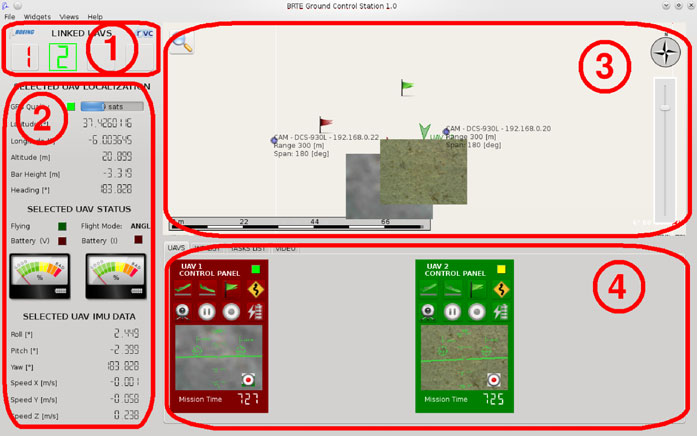
\includegraphics[width=\textwidth]{Ch2/gcs-perez}
	\caption[Ground control station main layout] {\small Ground control station main layout. Four main areas are numbered: (1) UAV selector, (2) detailed UAV information, (3) map area and (4) tab widget. Reprinted from \protect\shortciteA{perez2013ground}.}
	\label{fig:pixhawk}
\end{figure}
\FloatBarrier

\shortciteA{perez2013ground} prove that their system is successfully able to reduce the workload of the operator, fulfilling the goals of the project.

\section{Autopilot System}
\label{sect:autopilot}

There are already many existing autopilot systems, as covered by \citeA{chao2010autopilots}. Their study included both open source and proprietary autopilots. One of the most popular systems though nowadays is the Pixhawk. \citeA{meier2012pixhawk} says in their study:

\begin{quote}
    The PIXHAWK system is a flexible and computationally
strong research platform for autonomous micro air vehicles.
This system design, especially with a fast onboard com-
puter, is currently unmatched in the class of small-scale
MAVs.
\end{quote}

The system and communications architecture is designed for small-scale MAVs, and the MAVLink protocol in particular supports MAV-to-MAV communication, i.e. swarming (see above). 

Pixhawk PX4 and the ArduPilot are two of the most popular flight control software packages today. Both utilize the MAVLink protocol for communication between the GCS and the flight controller.

\begin{figure}[t]
	\centering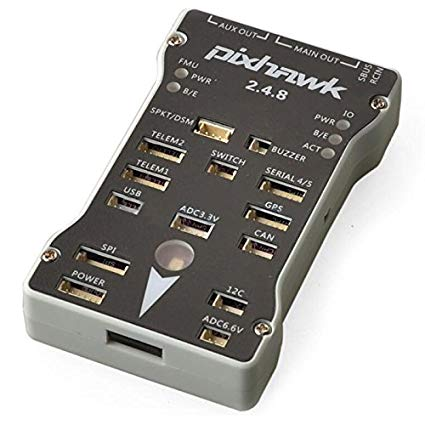
\includegraphics[width=0.3\textwidth]{Ch2/pixhawk}
	\caption{The Pixhawk 2.4.8. Reprinted from Amazon LLC.}
	\label{fig:pixhawk}
\end{figure}
\FloatBarrier

\section{Onboard Flight Computer}
Most UAVs are equipped with an onboard flight computer, containing a microcontroller and various peripherals. This allows drones to do heavy processing, such as computer vision, that the flight controller is under-equipped to handle. When thus equipped, drones can be identified as IoT devices, allowing for greater connectivity to other IoT devices.

There are a variety of micro-computers available on the market. A number of studies have been conducted to discover the performance of these devices \cite{benchmark} and \cite{maksimovic2014raspberry}. \citeA{maksimovic2014raspberry} found out that although the Pi performed less powerfully than the other considered hardware, it was the most cost-efficient and the most communication-friendly ``with support for a large number of input and output peripherals, and network communication'', making it ``the perfect platform for interfacing with many different devices and using in wide range of applications''.

The Raspberry Pi has also been tested in cloud computing applications. Some of the more reputable studes include those by \citeA{abrahamsson2013affordable} and \citeA{tso2013glasgow}.

\begin{figure}[t]
	\centering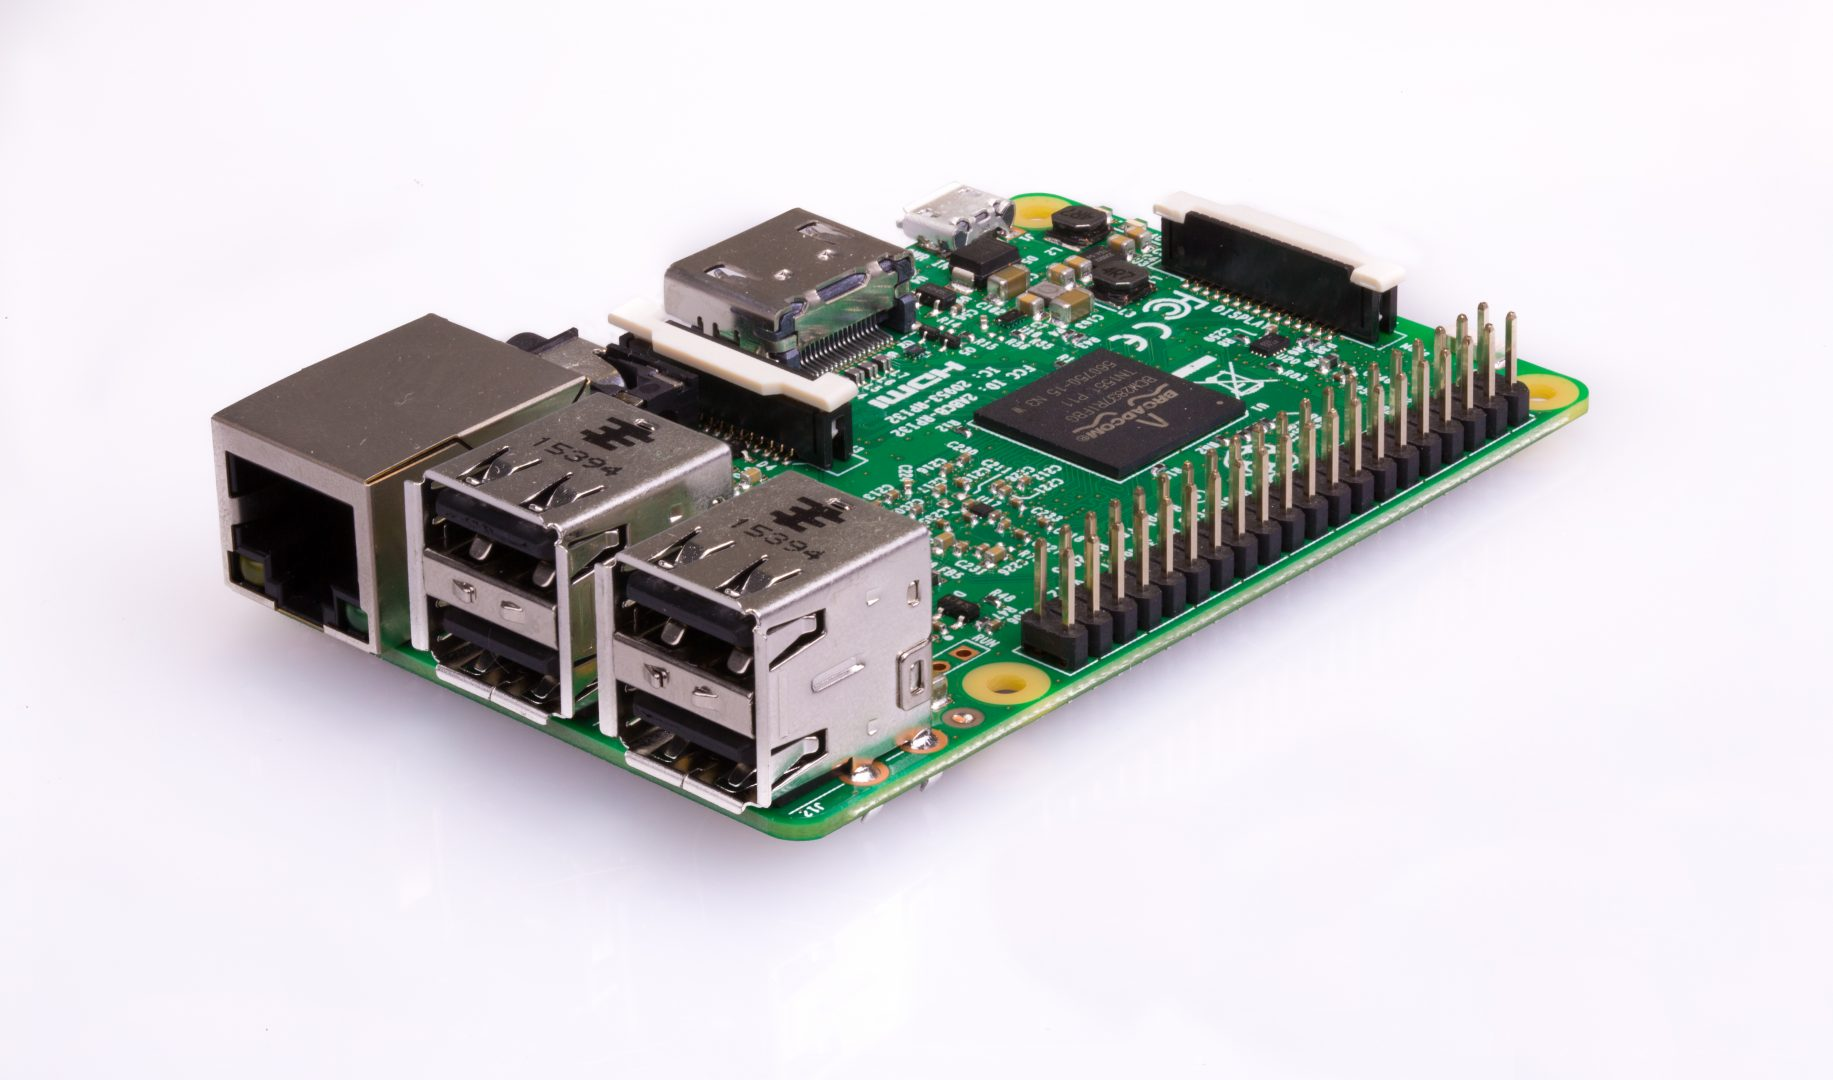
\includegraphics[width=0.5\textwidth]{Ch2/Raspberry-Pi-3}
	\caption{The Raspberry Pi 3 Model B. Reprinted from Raspberry Pi Foundation.}
	\label{fig:pixhawk}
\end{figure}
\FloatBarrier


% \shortciteA{yamato92hmm} apply the background subtraction 
% technique to extract blobs or human from a scene by the 
% following conditions:
% \[
% \begin{array}{lc}
%   {\rm if} & \left|{I_a (x,y) - I_b (x,y)}\right|< T,\;I_e (x,y) = 0 \\ 
%   {\rm else} & I_e (x,y) = I_a (x,y), 
% \end{array}
% \]
% where $I_e (x,y)$ is a human extracted image, $I_a (x,y)$ is an
% original image, $I_b (x,y)$ is a background image, and $T$ is a
% threshold. Figure~\ref{fig:mesh-feature} shows something. Some work also uses 
% mesh features~\shortcite{yamato92hmm}.

% % THE REASON ~ IS USED HERE BECAUSE WE TELL LATEX THAT THESE TWO WORDS SHOULD 
% % GO TOGETHER IN THE SAME LINE.

% \FloatBarrier

